%%%%%%%%%%%%%%%%%%%%%%%%%%%%%%%%%%%%%%%%%%%%%%%%%%%%%%%%%%%%%%%%%%%%%%%%%%%%%%%%
%
%   Semester project, fall term 2014
%   Author: Jakob Ehrl, born 01/24/91
%   Study program: Computer science, MA 1
%   
%   Professor Dr. Francesco Mondada
%   Assistant: Dr. Stefan Witwicki
%
%%%%%%%%%%%%%%%%%%%%%%%%%%%%%%%%%%%%%%%%%%%%%%%%%%%%%%%%%%%%%%%%%%%%%%%%%%%%%%%%%

\chapter{Central Processing}

\section{Setup of Processing Units}
Our robot is equipped with four different processing units that, together,
form a network of workers performing individual tasks. There is one master
node that receives sensor readings and lower level computation results from
the other nodes. This data is used to make decisions and finally send 
commands to control the actuators.


\subsection{Master Node}
An Odroid-C1 was used as master node. Similar to the well known Raspberry Pi,
this miniature computer has a Unix-based operating system and possesses numerous
ports such as USB, Ethernet, HDMI and various GPIO pins. We decided to use this
board instead of the Raspberry Pi, which is available in the virtual catalog,
because of the way we intended to design the network of processing units and 
data processing. With four USB ports instead of only two, four CPU cores and twice 
the amount of SDRAM, the Odroid-C1 allows to easily connect the other processing 
boards as well as a camera via USB. This allowed us to develop code in the same
way as if we were working on usual desktop computers. The need for a quad-core 
processor is justified since we aimed at separating the software into different 
modules that are supposed to run independently and in parallel. Pthreads were
used to process data from different inputs independently instead of in a single-loop program.

\subsection{Slaves}
Three Arduino boards were connected to the odroid via serial connection. The following
lists their responsibilities.

\begin{itemize}
    \item Arduino Micro 1
    \subitem control of brush motor
    \subitem data acquisition from five infrared sensors
    
    \item Arduino Micro 2
    \subitem data acquisition from compass 
    \subitem data acquisition from linear cameras

    \item Wild Thumper Controller
    \subitem control of wheels
    \subitem control of tailgate
\end{itemize}

\subsection{Communication}
To transmit data acquired by the Arduino boards and commands generated by the master,
we use the serial communication protocol. The micro controllers do not communicate with
each other. On both sides of the transmission there is a timed control loop that reads
and writes data at a frequency of 30 Hz. To reduce communication costs, all the available
data is first stored in a buffer. Only one message with all the collected commands/sensor
readings is transmitted per interval. This also allows us to filter sensor readings
and reduce communication overhead when the micro controller's control loop is faster 
than the master's planning phase.

\subsubsection{Message Format}
A message is composed of four ASCII characters. The first character being either an
upper- or lowercase character and the following three characters being digits with
leading zeros. Uppercase letters denote command IDs while lowercase letters denote
sensor IDs. Any number between 0 and 999 is allowed as respective value. 

\subsubsection{Limiting Factors}
Since Arduino boards have a small buffer for serial communication (64 bytes), continuous
communication causes a major bottleneck on the micro controllers. Therefore we 
had to limit the update frequency to 30 Hz and also limit the number of messages
that can be sent per iteration.


\section{Master Program Structure}
Code for the master node was written in C++ and designed in a modular way. The bottom
layer includes modules for sensing and acting. A middle layer provides easy access to 
the most recent sensor readings and also an interface for high-level control functions
by hiding actual actuator IDs and value checks behind human readable names such as
\texttt{setWheelSpeeds\{left, right\}}. The top level is where plans are made and 
commands are created. It offers both human interaction via keyboard or autonomous mode
through implementation of classes with access to the middle layer.

\subsection{Bottom Layer}

\subsubsection{Communication Module}
The class \texttt{Serial} implements low level serial communication between the master
node and any other node. The command line options \texttt{ard1, ard2, wtc} specify 
which entity the object shall represent. Their respective serial port locations must
be given as arguments after the option. For testing purposes, the program can be run
with three, two or no slave node connections.

Each connection to a slave is bounded in an object of class \texttt{Serial} having 
its own read and write buffer and its own thread. The communication loop inside a thread
is timed to read and write data at a frequency of 30 Hz to be congruent with the
micro controllers.

\subsubsection{Vision Module}
The class \texttt{Detector} implements the vision part of the robot. An object of this
class can be created from a connected camera or a single image (for development purposes).
It offers two options for image processing both working with color images. 

The first algorithm is based on a K-Means segmentation of the image. \texttt{BGPattern} allows
to create a desired number of color patterns that are later used to segment the image
into background and foreground. Given that there is a very limited number of possible
backgrounds in the arena (tiles, wood, grass, stones), the basic idea was to assign 
pixels within a certain distance to one of the background patterns. Pixels that are too
far from any of the clusters could then be considered as candidates for bottles.
Morphological operations (opening for noise reduction and dilation for region growing)
on the remaining binary image would eventually allow to classify regions of a certain
size and shape as bottles or obstacles.

The second algorithm is also based on the assumption of highly uniform background
patterns. It is implemented by the class \texttt{RangeFinder}. Assuming that the robot
is currently on drivable terrain, a small area in the lower part of the image (directly
in front of the robot) is used as sample pattern. This region is extended toward the
top of the image whilst the change in color is below a certain threshold. Boundaries
of this area are candidates for obstacles, bottles or sudden terrain changes. This 
option was found to generalize better than the first. A more detailed description is
given in the next section.

\subsection{Middle Layer}
The class \texttt{Brain} serves as a wrapper for sensing and acting modules. It 
communicates with objects from the bottom layer (\texttt{Serial, Detector}).
It provides access to all the measurements via the respective IDs defined in \texttt{defines.h}).
Getter and setter functions with respective value range checks allow to use the low-level 
functions from a more abstract point of view.

\subsection{Top Layer}
In order to control the robot either manually or from a custom controller, it is 
necessary to create objects from the lowest level and instantiate an object of type \texttt{Brain}.
An example for keyboard control can be found in \texttt{main.cpp}. Keys are directly mapped
to actions and therefore allow for remote control. Displaying visual output is optional
and can be disabled by the option \texttt{no\_cam}.

For autonomous mode, we tested two different approaches in the classes \texttt{Simulation} and
\texttt{Autonomous}.

\section{Vision}

\subsection{Camera}
A Playstation 3 Camera, an off-the-shelf USB camera, was mounted on a bridge on top of 
the robot covering a field of view from 10~cm to 250~cm in front of the robot and 
widths of 50~cm to 280~cm respectively. This camera was mainly chosen for its easily
modifiable Linux driver and its wide range of manual options such as exposure time,
gain and frame rate. Short exposure times at a constantly high frame rate were needed
to avoid blurred images. Since the camera is mounted almost 50~cm over ground, vibrations
and rough terrain (rocks) might cause blur and thereby make images useless.

\subsection{Algorithms}
Images taken by the camera were not only processed for object detection but also for 
the detection of terrain changes. Since our robot's bottle collection mechanism can only
work when it touches the ground, approaching the grass area or the rock barrier are
a particular danger causing the shovel to hook under the grass carpet or a rock.
The following explains the three key parts of our final algorithm.

\subsubsection{Preprocessing}
The input image is a $320 \times 240$ RGB image. 
An integral image is created from the original frame. Colors are not transformed into
gray scale. Therefore, the resulting integral image is still a three-channel matrix
of size $width + 1 \times height + 1$. The main advantage of integral images is 
that sums over rectangular pixel areas can be computed in constant time. The later
steps take advantage of this fact when computing average colors or applying filters.

\subsubsection{Terrain Segmentation}
Assuming that the image bottom captures drivable terrain, we want to grow determine 
future drivable terrain by growing the region captured in the image bottom toward
the top of the image.

For this purpose, the image is divided into 16 equally spaced columns of 20 pixels width.
In each column, we compute the average color over a region of 20 pixels height, hence 
a block size of $20 \times 20$ pixels. We then move up the image by half a block size
and re-compute the average color. We repeat this step until the distance between the
current and the preceding (half a block size lower) region is above a certain 
threshold. From an abstract point of view, we grow the drivable area by allowing a 
limited change in color. \figurename~\ref{fig:segmentation} shows the robots's point
of view when approaching the elevated area. For visualization the image is masked
with the result of the terrain segmentation step. Black means non-drivable.

Initially, we were planning on having a travel mode where the robot would move with the 
shovel slightly lifted. In order to still produce a good terrain segmentation,
we built in a mask that checks for the height of the white (high intensity) brush
in the image and consequently allows for vertical offsets of the central ten bars.

\begin{figure}
\center
\subfigure{
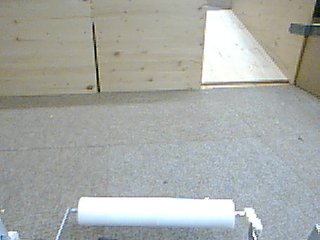
\includegraphics[width=0.45\textwidth]{figures/005.png}}
\hfill
\subfigure{
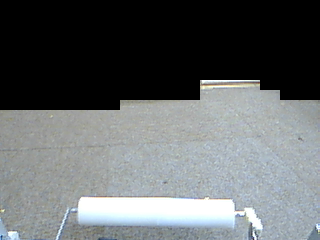
\includegraphics[width=0.45\textwidth]{figures/005-mask.png}}
\label{fig:segmentation}
\caption{Segmentation of drivable terrain.}
\end{figure}

\subsubsection{Detection of Terrain Transitions}
Given that terrain transitions in the arena are sharp straight lines, we can detect
those by fitting a regression line to the result of the segmentation step. Mostly, the
next encountered terrain does not span over the whole image and also only a small portion
of it is interesting to the robot -- the portion directly in front -- since it cannot
displace itself laterally.

Using OpenCV's \texttt{fitLine} function, we estimate a line in
2D over the central ten column heights of the previous step. Using the resulting
slope and offset, we compute the mean squared error of our estimate (summing up the 
squared differences between the true column heights and the predicted ones).
\figurename~\ref{fig:transition} shows the robot's point of view when approaching the
rock barrier with the expected terrain boundary denoted by the regression line in blue.

\begin{figure}
\centering
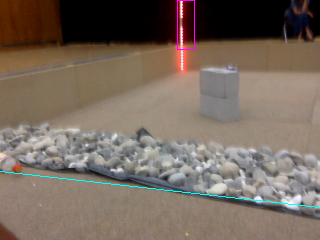
\includegraphics[width=0.45\textwidth]{figures/terrain-transition.png}
\label{fig:transition}
\caption{Regression line to terrain segmentation.}
\end{figure}

A low error means that the line fitting is appropriate and a terrain change is likely
while a high error signalizes a noisy boundary of the field of view. Boundary interruptions
(some columns lower than others) can be caused by obstacles, bottles or difficult lightning
conditions. Distance measures from the camera can help to detect 
terrain transitions as they cannot be seen by the infrared sensors. Obstacles,
however, can be detected by the infrared sensors. Consequently, range data from 
our infrared sensors should have higher weight then vision data and vision data
shall be used in cases where we have no response from infrared sensors.

\subsubsection{Beacon Detection}
Also seen in \figurename~\ref{fig:transition} is a purple frame around the light beacon.
Beacon detection can be handled in a very simple manner if the color does not need
to be determined. In our case, we decided to restrict to the pure detection without 
color classification since only the yellow beacon in the recycling zone was important
for our strategy. Having the compass and the information that there exists a beacon
in the current image, we can determine the corner we are approaching.

In our camera setup, beacons do always intersect with the upper image boundary.
We can therefore detect beacons by convolving the upper part of the image with a top-hat filter
moving from left to right. The pixel column with maximal response is considered a beacon
if its response exceeds a certain threshold in one of the three color channels. The filter
window height spans 20 pixel rows and 20 columns (5 negative columns on each side and 10 for
the central positive part). Taking the average over multiple image rows guarantees
that beacons are detected even though their intensity is not constantly high (due 
to the interruptions between LEDs). 

Once a tentative beacon column is found, the filter moves downward in the image.
In order to account for tilted beacons (or the camera not being mounted perfectly
horizontally), we allow for a small lateral motion of the filter window to the left
or right.

\subsubsection{Bottle Detection}
Bottles are detected as objects having high color differences with respect to the surrounding
area. Since the terrain boundaries are interrupted from such intensity changes, we find
bottles only on top of the 16 bars used for terrain segmentation. We designed a total of
nine different masks representing bottles at different distances and orientations.
Each mask is composed of square blocks of edge length 20 pixels. The blocks are stacked
(vertical bottle), placed aside (horizontal bottle) or placed with vertical and horizontal
offset ($45^\circ$) bottle. Depending on the distance (far, middle, close), blocks
do also overlap. \figurename~\ref{fig:bottles1} shows the result of the bottle detection
algorithm with three true positives and one false negative (left). Tests with low light
showed that the concept adapts well.

\begin{figure}
\center
\subfigure{
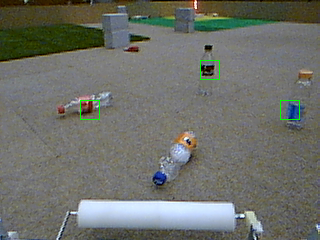
\includegraphics[width=0.45\textwidth]{figures/009.png}}
\hfill
\subfigure{
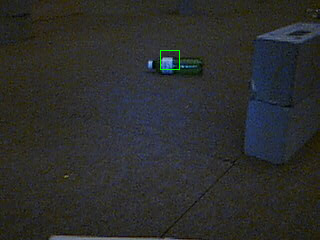
\includegraphics[width=0.45\textwidth]{figures/011.png}}
\label{fig:bottles1}
\caption{Bottle detection at different lightning conditions.}
\end{figure}


\subsubsection{Generated Data}
Output data generated from the above vision algorithms is collected in an object of type
\texttt{VisionMeasure} and handed to the \texttt{Brain}. It contains $x-$ and $y-$coordinates
in pixels, where $y=0$ is the bottom pixel row and $x=0$ is the horizontal center of the
image. There is also a vector of potential bottles with their respective coordinates,
slope and intersect of a regression line fit to the ten central bars and an error measure
reflecting confidence in the regression line.

Even though we could work with 3D data by calibrating the camera with respect to the
floor and compute distances and lateral offsets in cm, we decided to work with pixel
coordinates. We tried translating pixel coordinates into cm by measuring the field of view
of the camera and using the results for linear interpolation. However, this is eventually
only a scaling factor that can easier be taken care of when using the vision data. Hence,
we decided to transmit raw pixel measures and adjust accordingly in the control algorithm.

\subsection{Partial Results}
The terrain segmentation worked very well in most cases. Strong intensity changes on grass
produced poor segmentations. Dimming the ceiling light helped to avoid this. 
Our bottle detection had many false positives since it was very responsive to edges in
general. Rocks formed a particular problem. Taking into account the information
about terrain transitions might have helped to avoid these false positives since the 
rock barrier was detectable without any problems. However, this feature could not 
be added in time before the competition. 

Another problem came up during the competition. Our robot dropped off its bottle 
outside the recycling area due to a constant false positive beacon in the audience. 
High image intensities with a matching width for the top-hat filter.
It was the same place in both cases.
This means that the threshold was chosen too loosely and we could have avoided it.

\section{Control Algorithm}
The robot is a Braitenberg vehicle, meaning that depending on the type
of reading it receives steers its wheels toward or away from the perceived object.
Terrain classification as well as positions of obstacles and bottles detected through
vision will be added to guide the robot. Special behaviors as picking up a bottle,
returning home to the recycling station or releasing loaded bottles are planned.\\

In order to control the robot's locomotion a finite state machine has been developed .
In such a system to each state is associated a particular behavior of the robot that is triggered according to some predefined conditions.
The chosen states for our robot are shown in figure \ref{fig:FSM}\\

\begin{figure}
\centering
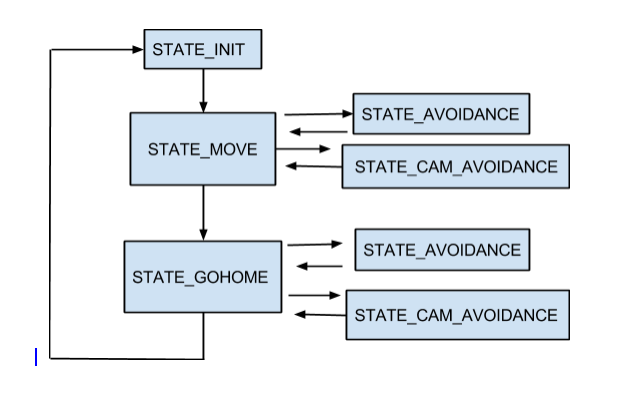
\includegraphics[width=0.8\textwidth]{FSM.png}
\caption{Finite State Machine of the robot.}
\label{fig:FSM}
\end{figure}

In the beginning the robot is in the STATE INIT. In this state the robot is initialized, meaning that it checks whether the tailgate for the bottles release is properly closed and if the brush is moving. After that the robot is directly moved to the STATE MOVE. This state represents the default behavior of the robot if no obstacles or changes of zone are detected. The robot simply moves straight ahead looking for bottles with the camera and, if it detects one of them, it steers toward the bottle in order to grasp it.

Once the bottle has been grasped, it is lifted up thanks to an IR sensor placed within the elevator and which detects if something is in it.
From this state the robot can pass to others three different behaviors according to some trigger conditions.\\

First of all, if the robot is within a range of 50 cm from an obstacle, that can be either a brick or a wall it enters the STATE AVOIDANCE.
In this state the speeds for the wheels are computed considering the robot as a Braitenberg's vehicle. This means that a bias speed is assigned to the wheels and then this value is modified exploiting a reactive architecture based on the IR sensors placed on the robot. Each sensor gives a value of the distance of the obstacles around the robot and afterwards this value is subtracted to 80 cm (maximum range of the IR sensor) in order to obtain a value that is bigger the closer an obstacle is to the robot. These values are then multiplied with weights properly chosen to obtain a smooth behavior of the robot while avoiding obstacles and also to modify the bias speeds to allow the robot to avoid having an impact with the brick or the wall.\\

The IR sensors are disposed in a symmetric way around the robot, in order to deal with the case in which the robot meets an obstacle perpendicular to it. A safety maneuver has been implemented consisting in making the robot drive backwards and turn of a small angle. This maneuver is activated when both the front IR sensors return a value of distance between a certain threshold that has been chosen of 50 cm.\\

After the robot has successfully avoided a possible impact it returns in STATE MOVE if the returned values from the sensors are bigger than a disable threshold, different from the enable one. The two thresholds are different otherwise the robot would just continuously switch between the two states getting stuck in its current location in the arena.\\

From the STATE MOVE the robot can also switch to the STATE CAM AVOIDANCE.
This state has as objective to allow the robot to identify a change of zone in the arena and avoid crossing it. This has been done because, even though the robot is capable of crossing all the possible areas, in case of failure of the procedure to lift up the robot's elevator the robot would simply risk to break part of its structure. As a consequence it has been chosen to avoid the bonus zones during the competition. This state exploits the information coming from the camera and if a change in the appearance of the terrain is detected, a safety maneuver like the one described above is performed.\\

Finally the robot can change from STATE MOVE to STATE GO HOME in order to bring the bottles to the reserved recycling area exploiting the information coming from the compass and then come back to the STATE MOVE. To avoid an impact during this process, from this state as well is possible for the robot to switch to the two states STATE AVOIDANCE and STATE CAM AVOIDANCE.




